% Add the listed directories to the search path
% (allows easy moving of files around later)
% these paths are searched AFTER local config kpsewhich

% *.sty, *.cls
\makeatletter
\def\input@path{{@resources/texlive/texmf-local/tex/latex/}
        ,{@resources/texlive/texmf-local/bibtex/bst/},
        ,{@resources/texlive/texmf-local/bibtex/bib/},
        ,{@local/}
        }
\makeatother
\makeatletter
\def\bibinput@path{{@resources/texlive/texmf-local/tex/latex/}
        ,{@resources/texlive/texmf-local/bibtex/bst/},
        ,{@resources/texlive/texmf-local/bibtex/bib/},
        ,{@local/}
        }
\makeatother
\documentclass[SolvingMicroDSOPs]{subfiles}
% econtexRoot gets obliterated by the documentclass command 
%\input{./.econtexRoot}\documentclass[SolvingMicroDSOPs]{subfiles}
\input{./.econtexRoot}\onlyinsubfile{% https://tex.stackexchange.com/questions/463699/proper-reference-numbers-with-subfiles
    \csname @ifpackageloaded\endcsname{xr-hyper}{%
      \externaldocument{\econtexRoot/SolvingMicroDSOPs}% xr-hyper in use; optional argument for url of main.pdf for hyperlinks
    }{%
      \externaldocument{\econtexRoot/SolvingMicroDSOPs}% xr in use
    }%
    \renewcommand\labelprefix{}%
    % Initialize the counters via the labels belonging to the main document:
}



% Get xrefs; only works properly if main file has already been successfully compiled
\onlyinsubfile{\externaldocument{SolvingMicroDSOPs}} 



\begin{document}
\hypertarget{method-of-moderation}{}
\section{The Method of Moderation}\label{sec:method-of-moderation}

The endogenous gridpoints method constructs a consumption function
$\Aprx{\cFunc}_{\prd}$ by interpolating a finite set of
$(\mNrm,\cNrm)$ pairs.  A practical problem arises when the
approximation must be evaluated at values of $\mNrm$ outside the
grid: na\"ive linear extrapolation can predict consumption so high
that precautionary saving turns negative, an economically impossible
result.

A solution, developed in \cite{method-of-moderation}, exploits the fact that the
true consumption function is bounded between two analytically
computable perfect-foresight rules.
\begin{itemize}
  \item \textbf{Optimist.} An agent who is certain that future income
  shocks will always equal their mean has human wealth
  $\hNrm_{\Cntn}$ and consumes
  \begin{equation}
    \cFuncAbove_{\prd}(\mNrm) \;=\;
      (\mNrm + \hNrm_{\Cntn})\,\MPCmin_{\prd},
      \label{eq:cFuncAboveBrief}
  \end{equation}
  where $\MPCmin_{\prd}$ is the minimal marginal propensity to
  consume of the corresponding perfect-foresight problem.
  \item \textbf{Pessimist.} An agent who assumes the worst possible
  income realisation in every future period has lower human wealth and
  a consumption floor at
  \begin{equation}
    \cFuncBelow_{\prd}(\mNrm) \;=\;
      (\mNrm - \Min{m}_{\prd})\,\MPCmin_{\prd},
      \label{eq:cFuncBelowBrief}
  \end{equation}
  where $\Min{m}_{\prd}$ is the natural borrowing constraint.
  \item \textbf{Realist.}  The true solution satisfies
  $\cFuncBelow_{\prd}(\mNrm) < \cFunc_{\prd}(\mNrm) <
  \cFuncAbove_{\prd}(\mNrm)$ for all $\mNrm$.
\end{itemize}

Because the realist's consumption always lies between these bounds, one can
define a \textit{moderation ratio}
\begin{equation}
  \omega_{\prd}(\mNrm) \;\equiv\;
    \frac{\cFunc_{\prd}(\mNrm) - \cFuncBelow_{\prd}(\mNrm)}
         {\cFuncAbove_{\prd}(\mNrm) - \cFuncBelow_{\prd}(\mNrm)}
    \;\in\; (0,1),
  \label{eq:modRteBrief}
\end{equation}
which measures how close the realist is to the optimist
($\omega=1$) versus the pessimist ($\omega=0$).  The key insight is
that the logit of this ratio,
$\log\!\bigl(\omega/(1-\omega)\bigr)$, is nearly linear
in $\mNrm$ and therefore easy to interpolate accurately.  Consumption
is recovered via the inverse transformation:
\begin{equation}
  \cFunc_{\prd}(\mNrm) \;=\;
    \cFuncBelow_{\prd}(\mNrm) \;+\;
    \frac{1}{1+e^{-\chi_{\prd}(\mNrm)}}
    \bigl(\cFuncAbove_{\prd}(\mNrm) - \cFuncBelow_{\prd}(\mNrm)\bigr),
  \label{eq:cFromChiBrief}
\end{equation}
where $\chi_{\prd} \equiv \log\!\bigl(\omega_{\prd}/(1-\omega_{\prd})\bigr)$
is the logit-transformed moderation ratio.  Since the recovered $\cFunc$
is automatically sandwiched between the bounds, the extrapolation problem
vanishes.

Figure~\ref{fig:IntExpFOCInvPesReaOptNeedHiPlot} illustrates the idea:
the realist consumption function (middle curve) is bounded above by the
optimist and below by the pessimist.

\begin{verbatimwrite}{./Figures/IntExpFOCInvPesReaOptNeedHiPlot.tex}
  \hypertarget{IntExpFOCInvPesReaOptNeedHiPlot}{}
  \begin{figure}
    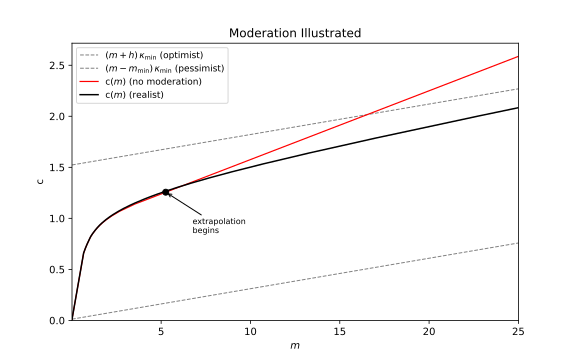
\includegraphics[width=6in]{./Figures/IntExpFOCInvPesReaOptNeedHiPlot}
    \caption[Moderation Illustrated]{Moderation Illustrated: $\cFuncBelow_{\prd-1} < \Aprx{\cFunc}_{\prd-1} < \cFuncAbove_{\prd-1}$}
    \label{fig:IntExpFOCInvPesReaOptNeedHiPlot}
  \end{figure}
\end{verbatimwrite}
  \hypertarget{IntExpFOCInvPesReaOptNeedHiPlot}{}
  \begin{figure}
    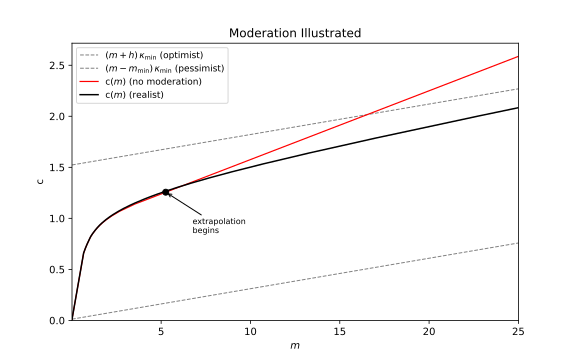
\includegraphics[width=6in]{./Figures/IntExpFOCInvPesReaOptNeedHiPlot}
    \caption[Moderation Illustrated]{Moderation Illustrated: $\cFuncBelow_{\prd-1} < \Aprx{\cFunc}_{\prd-1} < \cFuncAbove_{\prd-1}$}
    \label{fig:IntExpFOCInvPesReaOptNeedHiPlot}
  \end{figure}


The full treatment in \cite{method-of-moderation} extends the method with tighter
upper bounds, applies an analogous transformation to the value
function, and shows how to handle stochastic returns and Hermite
interpolation refinements.

\end{document}
